\documentclass[14pt, a4paper]{article}
\usepackage{fullpage}
\usepackage[top=2cm, bottom=2cm, left=2.5cm, right=2cm]{geometry}
\usepackage{amsmath,amsthm,amsfonts,amssymb,amscd}
\usepackage{fancyhdr}
\usepackage{fixltx2e}
\usepackage{mathrsfs}
\usepackage{listings}
\usepackage{color}
\usepackage{relsize}
\usepackage{graphicx}
\usepackage[utf8]{inputenc}
\usepackage[T1]{fontenc}
\usepackage[english, russian]{babel}

\definecolor{dkgreen}{rgb}{0,0.6,0}
\definecolor{gray}{rgb}{0.5,0.5,0.5}
\definecolor{mauve}{rgb}{0.58,0,0.82}

\DeclareMathSizes{14}{24}{18}{12}

\lstset{frame=tb,
  language=Python,
  aboveskip=3mm,
  belowskip=3mm,
  showstringspaces=false,
  columns=flexible,
  basicstyle={\small\ttfamily},
  numbers=none,
  numberstyle=\tiny\color{gray},
  keywordstyle=\color{blue},
  commentstyle=\color{dkgreen},
  stringstyle=\color{mauve},
  breaklines=true,
  breakatwhitespace=true,
  tabsize=3
}

\renewcommand{\thesection}{\arabic{section}.}
\renewcommand{\thesubsection}{\thesection\arabic{subsection}.}
\renewcommand{\thesubsubsection}{\thesubsection\arabic{subsubsection}.}

\begin{document}
\pagenumbering{gobble}
\begin{titlepage}
\begin{center}
\large{БЕЛОРУССКИЙ ГОСУДАРСТВЕННЫЙ УНИВЕРСИТЕТ 

ФАКУЛЬТЕТ ПРИКЛАДНОЙ МАТЕМАТИКИ И ИНФОРМАТИКИ

КАФЕДРА ВЫЧИСЛИТЕЛЬНОЙ МАТЕМАТИКИ}
\end{center}
\vspace*{\fill}
\begin{center}
Лабораторная работа 8

\large{\textbf{Применение многочлена Лагранжа для интерполирования функции}}

Вариант 7
\end{center}
\begin{flushright}
\textbf{Выполнил:}

Журик Никита Сергеевич \\ 2 курс, 6 группа

\textbf{Преподаватель:}

Будник Анатолий Михайлович
\end{flushright}
\vspace*{\fill}
\begin{center}
Минск, 2019
\end{center}
\end{titlepage}

\tableofcontents
\newpage

\newpage
\pagenumbering{arabic}

  \section{Постановка задачи}
    \begin{enumerate}
      \item
      При помощи построения многочлена Лагранжа выполнить интерполирование данной функции $f(x)$;
      \item
      Вычислить теоретическую оценку и действительную невязку интерполирования;
      \item
      Проанализировать результаты и сравнить с методом наименьших квадратов.
    \end{enumerate}
  \section{Алгоритм решения}
  \begin{itemize}
     \item
     Рассмотрим интерполирование исходной функции $f(x) = 1.7e^{-x} - 0.7lnx$ алгебраическим многочленом степени не выше $n$: $P_n(x) = \sum\limits_{i = 0}^n c_ix^i$ на сетке узлов $x_i = 1 + ih, i = \overline{1, 10}, h = \frac{1}{10}$.
     \item
     Тогда воспользуемся формулой Лагранжа для интерполяционного многочлена: \begin{align}P_n(x) &= \sum\limits_{i=0}^n l_i(x)f(x_i) \\ P_n(x) &= \sum\limits_{i = 0}^n \frac{\omega_{n+1}(x)}{(x-x_i)\omega_{n+1}'(x_i)}f(x_i) \\ P_n(x) &= \sum\limits_{i=0}^n \frac{(x-x_0)\dots(x-x_{i-1})(x-x_{i+1})\dots(x-x_n)}{(x_i-x_0)\dots(x_i-x_{i-1})(x_i-x_{i+1})\dots(x_i-x_n)}f(x_i)\end{align}
     (В (2) $\omega_{n+1}(x) = \prod\limits_{i=0}^n (x-x_i)$).
     \item
     Для априорной оценки точности интерполирования на всём промежутке воспользуемся формулой остатка интерполирования в форме Лагранжа:
     \begin{equation}r_n(x) = \frac{f^{(n+1)}(\xi)}{(n+1)!}\omega_{n+1}(x) \implies |r_n(x)| \leq \frac{\max\limits_{\xi \in [a, b]} |f^{(n+1)}(\xi)|}{(n+1)!}|\omega_{n+1}(x)| \end{equation}
  \end{itemize}
  \section{Листинг программы}
  Для реализации алгоритма был использован Python и библиотеки numpy и matplotlib.

\begin{lstlisting}
#Lagrange.py

import numpy as np
from math import exp, log, factorial
import matplotlib.pyplot as plt

a = 1.0
b = 2.0
N = 10
delta = (b - a) / N
alpha = 1.7

points = [a + i * delta for i in range(N + 1)]

def f(x):
    return alpha * exp(-x) + (1 - alpha) * log(x)

def fDerivN1(x):
    return -1 ** (N + 1) * alpha * exp(-x) + (1 - alpha) * (-1 ** N) * factorial(N - 1) / x ** N

def maxDerivN1(samples):
    space = np.linspace(a, b, samples)
    return np.max(np.abs(np.array([(fDerivN1(x)) for x in space], dtype=np.double)))

def omega(k, x):
    global points
    result = 1
    for i in range(N + 1):
        if i != k:
            result *= (x - points[i])
    return result

def denominator(k):
    global points
    result = 1
    for i in range(N + 1):
        if i != k:
            result *= (points[k] - points[i])
    return result

def l(k):
    return lambda x: omega(k, x) / denominator(k)

def LagrangePolynomial(x):
    result = 0
    for i in range(N + 1):
        result += l(i)(x) * f(points[i])
    return result

def deficiency(x):
    return maxDerivN1(10000) * omega(-1, x) / factorial(N + 1)

def plotDifference(samples):
    space = np.linspace(a, b, samples)
    plt.plot(space, np.zeros(np.shape(space)))
    plt.plot(space, np.array([LagrangePolynomial(x) - f(x) for x in space], dtype=np.double))
    plt.show()
    
if __name__ == '__main__':

    check = [points[0] + delta / 2.6, 
             points[5] + delta / 2.6,
             points[9] + delta / 2.6]
    
    [print("Pn({0}) = {1}".format(x, LagrangePolynomial(x))) for x in check]
    print()
    [print("rn({0}) = {1}".format(x, LagrangePolynomial(x) - f(x))) for x in check]
    print()

    print("M: " + str(maxDerivN1(10000)))
    print()
    
    print("Expected deficiency: " + 
          str(np.max(np.abs(np.array([(deficiency(x)) for x in check], dtype=np.double)))))
    
    space = np.linspace(a, b, 1000)
    print("Real deficiency on whole interval: " + 
          str(np.max(np.abs(np.array([(LagrangePolynomial(x) - f(x)) for x in space], dtype=np.double)))))
    print()
    
    print("Real deficiency on control points: " + 
          str(np.max(np.abs(np.array([(LagrangePolynomial(x) - f(x)) for x in check], dtype=np.double)))))
    
    plotDifference(1000)
\end{lstlisting}

  \section{Вывод программы}
\begin{verbatim}
Pn(1.0384615384615385) = 0.5753798661146213
Pn(1.5384615384615385) = 0.06346095167693702
Pn(1.9384615384615385) = -0.21865340262681945

rn(1.0384615384615385) = 4.9781948563421e-09
rn(1.5384615384615385) = -3.9230313442217835e-11
rn(1.9384615384615385) = -1.66610031326897e-09

M: 254015.37460495

Expected deficiency: 2.4883946749229354e-08
Real deficiency on whole interval: 5.350829113126565e-09

Real deficiency on control points: 4.9781948563421e-09
\end{verbatim}
\begin{figure}[h!]
  \center
  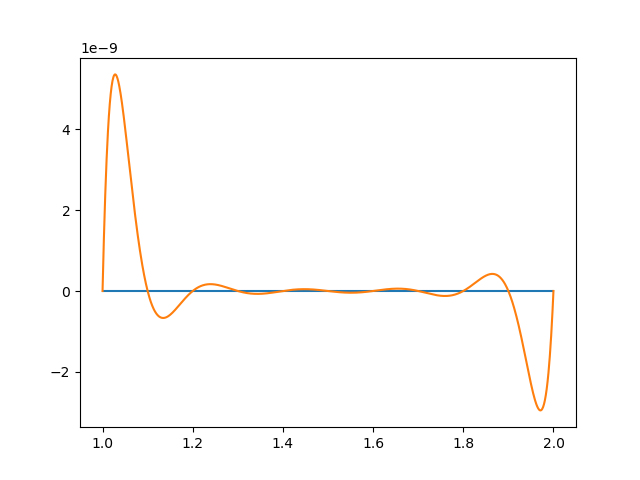
\includegraphics[width=0.6\linewidth]{LagrangeDiff.png}
  \caption{Невязка интерполирования}
\end{figure}

  \section{Выводы}
  \begin{itemize}
  \item
  При интерполировании при помощи многочлена Лагранжа была получена теоретическая оценка невязки $r_{Lagr_{theor}} = 2.4883946749229354e-08$, в действительности же максимальная невязка на всём промежутке оказалась равной $r_{Lagr_{real}} = 5.350829113126565e-09$, а в контрольных точках - $r_{Lagr_{control}} = 4.9781948563421e-09$.
  \item
  Сравним многочлен Лагранжа с МНК. В МНК невязка в контрольных точках составила $r_{LSQ_{control}} = 9.374749135870886e-06$, что значительно больше полученной в данном методе. Это связано с тем, что матрица Гильберта плохо обусловлена (для $n=5$ число обусловленности имеет порядок $10^{11}$. Таким образом, посредством многочлена Лагранжа можно добиться большей точности, чем при приближении функции методом наименьших квадратов.
  \item
  Глядя на график невязки, можно заметить, что невязка в середине отрезка меньше невязки на концах, что, как и в методе наименьших квадратов, связано с тем, что за пределами отрезка интерполирования многочлен Лагранжа не совпадает с исходной функцией и невязка значительно увеличивается.
  \end{itemize}

\end{document}